% This is uvh5_memo.tex, a memo on the uvh5 format
% The minted package is used for syntax highlighting of code, and requires the
% pygments package to be installed. pdflatex also needs to be invoked with the
% -shell-escape option. To compile this document:
%   $ pdflatex -shell-escape uvh5_memo.tex
% This should compile the document into uvh5_memo.pdf

\documentclass[11pt, oneside]{article}
\usepackage{geometry}
\geometry{letterpaper}
\usepackage{graphicx}
\usepackage[titletoc,toc,title]{appendix}							
\usepackage{amssymb}
\usepackage{physics}
\usepackage{array}
\usepackage{makecell}

\usepackage{hyperref} 
\hypersetup{
    colorlinks = true
}

\usepackage{cleveref}
\crefformat{footnote}{#2\footnotemark[#1]#3}
\usepackage{minted}

\title{Memo: UVH5 file format}
\author{Paul La Plante, and the pyuvdata team}
\date{November 28, 2018\\
Revised April 2, 2021}

\begin{document}
\maketitle
\tableofcontents
\section{Introduction}
\label{sec:intro}
This memo introduces a new HDF5\footnote{\url{https://www.hdfgroup.org/}}-based
file format of a UVData object in
\verb+pyuvdata+\footnote{\url{https://github.com/HERA-Team/pyuvdata}}, a python
package that provides an interface to interferometric data. Here, we describe
the required and optional elements and the structure of this file format, called
\textit{UVH5}.

Note that this file format is specifically designed to represent UVData
objects. Other HDF5-based datasets for radio interferometers, such as
katdal\footnote{\url{https://github.com/ska-sa/katdal}} or
HDFITS\footnote{\url{https://github.com/telegraphic/fits2hdf}} \textit{are not
  compatible} with the standard as defined here. We refer the reader to the
documentation of those other formats to find out more about them.

We assume that the user has a working knowledge of HDF5 and the associated
python bindings in the package \verb+h5py+\footnote{\url{https://www.h5py.org/}}, as
well as UVData objects in pyuvdata. For more information about HDF5, please
visit \url{https://portal.hdfgroup.org/display/HDF5/HDF5}. For more information
about the parameters present in a UVData object, please visit
\url{http://pyuvdata.readthedocs.io/en/latest/uvdata_parameters.html}. An
example for how to interact with UVData objects in pyuvdata is available at
\url{http://pyuvdata.readthedocs.io/en/latest/tutorial.html}.

Note that throughout the documentation, we assume a row-major convention (i.e.,
C-ordering) for the dimension specification of multi-dimensional arrays. For
example, for a two-dimensional array with shape ($N$, $M$), the $M$-dimension is
varying fastest, and is contiguous in memory. This convention is the same as
Python and the underlying C-based HDF5 library. Users of languages with the
opposite column-major convention (i.e., Fortran-ordering, seen also in MATLAB
and Julia) must transpose these axes.

\section{Overview}
\label{sec:overview}
A UVH5 object contains the interferometric data from a radio telescope, as well
as the associated metadata necessary to interpret it. A UVH5 file contains two
primary HDF5 groups: the \verb+Header+ group, which contains the metadata, and
the \verb+Data+ group, which contains the data itself, the flags, and
information about the number of samples corresponding to the data. Datasets in
the \verb+Data+ group are also typically passed through HDF5's compression
pipeline, to reduce the amount of on-disk space required to store the data.
However, because HDF5 is aware of any compression applied to a dataset, there is
little that the user has to explicitly do when reading data. For users
interested in creating new files, the use of compression is not strictly
required by the UVH5 format, again because the HDF5 file is self-documenting in
this regard. However, be warned that most UVH5 files ``in the wild'' typically
feature compression of datasets in the \verb+Data+ group.

In the disucssion below, we discuss required and optional datasets in the
various groups. We note in parenthesis the corresponding attribute of a UVData
object. Note that in nearly all cases, the names are coincident, to make things
as transparent as possible to the user.

\section{Header}
\label{sec:header}
The \verb+Header+ group of the file contains the metadata necessary to interpret
the data. We begin with the required parameters, then continue to optional
ones. Unless otherwise noted, all datasets are scalars (i.e., not arrays). The
precision of the data type is also not specified as part of the format, because
in general the user is free to set it according to the desired use case (and
HDF5 records the precision and endianness when generating datasets). When using
the standard \verb+h5py+-based implementation in pyuvdata, this typically
results in 32-bit integers and double precision floating point numbers. Each
entry in the list contains \textbf{(1)} the exact name of the dataset in the
HDF5 file, in boldface, \textbf{(2)} the expected datatype of the dataset, in
italics, \textbf{(3)} a brief description of the data, and \textbf{(4)} the name
of the corresponding attribute on a UVData object. Note that unlike in other
formats, names of HDF5 datasets can be quite long, and so in most cases the name
of the dataset corresponds to the name of the UVData attribute.

Note that string datatypes should be handled with care. See
Appendix~\ref{appendix:strings} for appropriately defining them for
interoperability between different HDF5 implementations.

\subsection{Required Parameters}
\label{sec:req_params}
\begin{itemize}
\item \textbf{latitude}: \textit{float} The latitude of the telescope site, in
  degrees. (\textit{latitude})
\item \textbf{longitude}: \textit{float} The longitude of the telescope site, in
  degrees. (\textit{longitude})
\item \textbf{altitude}: \textit{float} The altitude of the telescope site, in
  meters. (\textit{altitude})
\item \textbf{telescope\_name}: \textit{string} The name of the telescope used
  to take the data. The value is used to check that metadata is self-consistent
  for known telescopes in pyuvdata. (\textit{telescope\_name})
\item \textbf{instrument}: \textit{string} The name of the instrument, typically
  the telescope name. (\textit{instrument})
\item \textbf{object\_name}: \textit{string} The name of the object tracked by
  the telescope. For a drift-scan antenna, this is typically
  ``zenith''. (\textit{object\_name})
\item \textbf{history}: \textit{string} The history of the data
  file. (\textit{history})
\item \textbf{phase\_type}: \textit{string} The phase type of the
  observation. Should be ``phased'' or ``drift''. Note that ``drift'' in this
  context more accurately means ``unphased'', in that baselines are computing
  using ENU coordinates, without any $w$-projection. Any other value is treated as
  an unrecognized type. (\textit{phase\_type})
\item \textbf{Nants\_data}: \textit{int} The number of antennas that data in the
  file corresponds to. May be smaller than the number of antennas in the
  array. (\textit{Nants\_data})
\item \textbf{Nants\_telescope}: \textit{int} The number of antennas in the
  array. May be larger than the number of antennas with data corresponding to
  them. (\textit{Nants\_telescope})
\item \textbf{ant\_1\_array}: \textit{int} An array of the first antenna numbers
  corresponding to baselines present in the data. All entries in this array must exist
  in the antenna\_numbers array. This is a one-dimensional
  array of size Nblts. (\textit{ant\_1\_array})
\item \textbf{ant\_2\_array}: \textit{int} An array of the second antenna numbers
  corresponding to baselines present in the data. All entries in this array must exist
  in the antenna\_numbers array. This is a one-dimensional
  array of size Nblts. (\textit{ant\_2\_array})
\item \textbf{antenna\_numbers}: \textit{int} An array of the numbers of the antennas
  present in the radio telescope (note that these are not indices, they do not need to start at zero
  or be continuous). This is a one-dimensional array of size
  Nants\_telescope. Note there must be one entry for every unique antenna in
  ant\_1\_array and ant\_2\_array, but there may be additional
  entries. (\textit{antenna\_names})
\item \textbf{antenna\_names}: \textit{string} An array of the names of antennas
  present in the radio telescope. This is a one-dimensional array of size
  Nants\_telescope. Note there must be one entry for every unique antenna in
  ant\_1\_array and ant\_2\_array, but there may be additional
  entries. (\textit{antenna\_names})
\item \textbf{Nbls}: \textit{int} the number of baselines present in the
  data. For full cross-correlation data (including auto-correlations), this
  should be Nants\_data$\times$(Nants\_data+1)/2. (\textit{Nbls})
\item \textbf{Nblts}: \textit{int} The number of baseline-times (i.e., the
  number of spectra) present in the data. Note that this value need not be equal
  to Nbls $\times$ Ntimes. (\textit{Nblts})
\item \textbf{Nspws}: \textit{int} The number of spectral windows present in the
  data. (\textit{Nspws})
\item \textbf{Nfreqs}: \textit{int} The total number of frequency channels in
  the data across all spectral windows. (\textit{Nfreqs})
\item \textbf{Npols}: \textit{int} The number of polarization products in the
  data. (\textit{Npols})
\item \textbf{Ntimes}: \textit{int} The number of time samples present in the
  data. (\textit{Ntimes})
\item \textbf{uvw\_array}: \textit{float} An array of the uvw-coordinates
  corresponding to each observation in the data. This is a two-dimensional array of
  size (Nblts, 3). Units are in meters. (\textit{uvw\_array})
\item \textbf{time\_array}: \textit{float} An array of the Julian Date
  corresponding to the temporal midpoint of the corresponding baseline's
  integration. This is a one-dimensional array of size
  Nblts. (\textit{time\_array})
\item \textbf{integration\_time}: \textit{float} An array of the duration in
  seconds of an integration. This is a one-dimensional array of size
  Nblts. (\textit{integration\_time})
\item \textbf{freq\_array}: \textit{float} An array of all the frequencies (for
  all spectral windows) stored in the file in Hertz. This is a one-dimensional
  array of size (Nfreqs). (\textit{freq\_array})
\item \textbf{channel\_width}: \textit{float} The width of frequency channels in
  the file in Hertz. This is a one-dimensional array of size
  (Nfreqs). (\textit{channel\_width})
\item \textbf{spw\_array}: \textit{int} An array of the spectral windows in the
  file. This is a one-dimensional array of size Nspws. (\textit{spw\_array})
\item \textbf{flex\_spw}: \textit{python bool}\footnote{Note that this is
    \textit{not} the same as the \texttt{H5T\_NATIVE\_HBOOL} type; instead, it
    is an \texttt{H5Tenum} type, with an explicit \texttt{TRUE} and
    \texttt{FALSE} value. Such a type is created automatically when using
    \texttt{h5py}, both for Python \texttt{bool} and numpy \texttt{np.bool\_}
    types. See Appendix~\ref{appendix:boolean} for an example of how to define
    this in C. Such a definition should follow analogously in other languages.}
  Whether the data are saved using flexible spectral windows. If more than one
  spectral window is present in the data, this must be \texttt{True}. See
  Sec.~\ref{sec:flex_spw} for a discussion of the details. (\textit{flex\_spw})
\item \textbf{polarization\_array}: \textit{int} An array of the polarizations
  contained in the file. This is a one-dimensional array of size Npols. Note
  that the polarizations should be stored as an integer, and use the convention
  defined in AIPS Memo 117. (\textit{polarization\_array})
\item \textbf{antenna\_positions}: \textit{float} An array of the antenna
  coordinates relative to the reference position of the radio telescope array,
  which is implicitly defined by the \textit{latitude}, \textit{longitude}, and
  \textit{altitude} (LLA) parameters. More explicitly, these are the ECEF
  coordinates of individual antennas minus the ECEF coordinates of the reference
  telescope position, such that the telescope position plus the values stored in
  \textit{antenna\_positions} equals the position of individual elements in
  ECEF. The conversion between LLA and ECEF is given by WGS84. This is a
  two-dimensional array of size (Nants\_telescope,
  3). (\textit{antenna\_positions})
\item \textbf{version}: \textit{string} The version of the HDF5 file. The latest
  version (and the one described in this memo) is Version 1.0. Note it should be
  a string, such as \verb+`1.0'+. See Sec.~\ref{sec:version_history} for the
  version history of the HDF5 specification. (\textit{version})
\end{itemize}

\subsection{Optional Parameters}
\label{sec:opt_params}
\begin{itemize}
\item \textbf{flex\_spw\_id\_array}: \textit{int} The mapping of individual
  channels along the frequency axis to individual spectral windows, as listed in
  the \textit{spw\_array}. This is a one-dimensional array of size
  (Nfreqs). Note this is \textbf{required} if the file uses flexible
  spectral windows (see
  Sec.~\ref{sec:flex_spw}). (\textit{flex\_spw\_id\_array})
\item \textbf{dut1}: \textit{float} DUT1 (google it), in seconds. AIPS 117 calls
  it \verb+UT1UTC+. (\textit{dut1})
\item \textbf{earth\_omega}: \textit{float} Earth's rotation rate in degrees per
  day. Note the difference in units, which is inherited from the way this
  quantity is handled in UVFITS datasets (AIPS 117 calls it \verb+DEGPDY+).
  (\textit{earth\_omega})
\item \textbf{gst0}: \textit{float} Greenwich sidereal time at midnight on
  reference date, in degrees. AIPS 117 calls it \verb+GSTIA0+ (\textit{gst0})
\item \textbf{rdate}: \textit{string} Date for which GST0 (or whichever time
  saved in that field) applies. Note this is different from how UVFITS handles
  this quantity, which is saved as a float rather than a string. The user is
  encouraged to ensure it is being handled self-consistently for their desired
  application. (\textit{rdate})
\item \textbf{timesys}: \textit{string} Time system. pyuvdata currently only
  supports UTC. (\textit{timesys})
\item \textbf{x\_orientation}: \textit{string} The orientation of the x-arm of a
  dipole antenna. It is assumed to be the same for all antennas in the
  dataset. For instance, ``East'' or ``North'' may be
  used. (\textit{x\_orientation}).
\item \textbf{antenna\_diameters}: \textit{float} An array of the diameters of
  the antennas in meters. This is a one-dimensional array of size
  (Nants\_telescope). (\textit{Nants\_telescope})
\item \textbf{phase\_center\_catalog}: A series of nested datasets, similar to
a dict in python. The top level keys are strings giving the phase center
catalog names. The next level keys must include:
	\begin{itemize}
	\item \textbf{cat\_id}: \textit{int} The phase center catalog ID number,
	which is used to identify which baseline times are phased to which
	phase center via the phase\_center\_id\_array.
	\item \textbf{cat\_type}: \textit{string} One of four allowed values:
	\textbf{(1)} sidereal, \textbf{(2)} ephem, \textbf{(3)} driftscan,
	\textbf{(4)} unprojected.
  	Sidereal means a phase center that is fixed in RA and Dec.
	Ephem means a phase center that has an RA and Dec that
	moves with time.
	Driftscan means a phase center with a fixed azimuth and
	elevation (note that this includes w-projection, even at zenith).
	Unprojected means no phasing, including w-projection, has been applied.
  
	\end{itemize}
  
\item \textbf{uvplane\_reference\_time}: \textit{int} The time at which the
  phase center is normal to the chosen UV plane for phasing. Used for
  interoperability with the FHD
  package\footnote{\url{https://github.com/EoRImaging/FHD}}.
\item \textbf{lst\_array}: \textit{float} An array corresponding to the local
  sidereal time of the center of each observation in the data in units of
  radians. If it is not specified, it is calculated from the latitude/longitude
  and the time\_array. Saving it in the file can be useful for files with many
  values in the \textit{time\_array}, which would expensive to
  recompute. (\textit{lst\_array})
\end{itemize}

\subsection{Extra Keywords}
\label{sec:extra_keywords}
UVData objects support ``extra keywords'', which are additional bits of
arbitrary metadata useful to carry around with the data but which are not
formally supported as a reserved keyword in the \verb+Header+. In a UVH5 file,
extra keywords are handled by creating a datagroup called \verb+extra_keywords+
inside the \verb+Header+ datagroup. In a UVData object, extra keywords are
expected to be scalars, but UVH5 makes no formal restriction on this. Also, when
possible, these quantities should be HDF5 datatypes, to support interoperability
between UVH5 readers. Inside of the extra\_keywords datagroup, each extra
keyword is saved as a key-value pair using a dataset, where the name of the
extra keyword is the name of the dataset and its corresponding value is saved in
the dataset. Though the use of HDF5 attributes can also be used to save
additional metadata, it is not recommended, due to the lack of support inside of
pyuvdata for ensuring the attributes are properly saved when writing out.


\section{Data}
\label{sec:data}
In addition to the \verb+Header+ datagroup in the root namespace, there must be
one called \verb+Data+. This datagroup saves the visibility data, flags, and
number of samples corresponding to each entry. All three datasets must be
present in a valid UVH5 file. They are also all expected to be the same shape:
(Nblts, Nfreqs, Npols). Note that due to the intermixing of the baseline and
time axes, it is \textit{not} required for data to exist for every baseline and
time in the file. This behavior is similar to UVFITS and MIRIAD file
formats. Also note that there is no explicit ordering required for the
baseline-time axis. A common ordering is to write the data in ``correlator
order'', and have all baselines for a single time $t_i$, followed by all
baselines for the next time $t_{i+1}$, etc. However, this is merely a
convention, and is not explicitly required for the UVH5 format.

\subsection{Visdata Dataset}
\label{sec:visdata}
The visibility data is saved as a dataset named \verb+visdata+. It should be a
3-dimensional, complex-type dataset with shape (Nblts, Nfreqs, Npols). Most
commonly this is saved as an 8-byte complex number (a 4-byte float for the real
and imaginary parts), though some flexibility is possible. 16-byte complex
floating point numbers (composed of two 8-byte floats), as well as 8-byte
complex integers (two 4-byte signed integers), are also common. In all cases, a
compound datatype is defined, with an \verb+`r'+ field and an \verb+`i'+ field,
corresponding to the real and imaginary parts, respectively. The real and
imaginary types must also be the same datatype. For instance, they should both
be 8-byte floating point numbers, or 32-bit (4-byte) integers. Mixing datatypes
between the real and imaginary parts is not allowed.

Using \verb+h5py+, the datatype for \verb+visdata+ can be specified as
\verb+`c8'+ (8-byte complex numbers, corresponding to the \verb+np.complex64+
datatype) or \verb+`c16'+ (16-byte complex numbers, corresponding to the
\verb+np.complex128+ datatype) out-of-the-box, with no special handling by the
user. \verb+h5py+ transparently handles the definition of the compound
datatype. For examples of how to handle complex integer datatypes in
\verb+h5py+, see Appendix~\ref{appendix:integers}.

\subsubsection{Conjugation Convention}
A cross-correlation between two antennas is defined by the baseline connecting
them, and the conjugation of one of the input data streams. Accordingly, the
\textit{uvw} coordinates and the conjugation of the visibility data are
interconnected, based on the definition of one's coordinate system. For UVH5
files, it is assumed that the convention for the Radio Interferometer
Measurement Equation (RIME) of a visibility $\mathcal{V}$ for antennas $i$ and
$j$ is as follows \cite{tms}:
\begin{equation}
\mathcal{V}(u_j - u_i, v_j - v_i) = \int \dd{l} \dd{m} I(l, m) g_i(l, m) e^{-2\pi i (u_i l + v_i m)} g_j^*(l, m) e^{2\pi i (u_j l + v_j m)}.
\end{equation}
That is, the baseline vector defined by the $uvw$ coordinates is directed from
antenna $i$ to antenna $j$ (so the baseline vector can be computed as
$\vb{r_j} - \vb{r_i}$, where $\vb{r}$ is the position vector of a given
antennas), and the data corresponding to antenna $j$ is conjugated. Note that if
a file is generated with the opposite convention, it is usually sufficient to
multiply $uvw$ coordinates by $-1$ to generate a self-consistent dataset, as
well as conjugating the data in the \verb+data_array+.

\subsection{Flags Dataset}
\label{sec:flags}
The flags corresponding to the data are saved as a dataset named
\verb+flags+. It is a 3-dimensional, boolean-type dataset with shape (Nblts,
Nfreqs, Npols). Values of True correspond to instances of flagged data, and
False is non-flagged. Note that the boolean type of the data is \textit{not} the
HDF5-provided \verb+H5T_NATIVE_HBOOL+, and instead is defined to conform to the
\verb+h5py+ implementation of the numpy boolean type. When creating this dataset
from \verb+h5py+, one can specify the datatype as \verb+np.bool_+. Behind the
scenes, this defines an HDF5 enum datatype. See Appendix~\ref{appendix:boolean}
for an example of how to write a compatible dataset from C.

As with the nsamples dataset discussed below, compression is typically applied
to the flags dataset. The LZF filter (included in all HDF5 libraries) provides a
good compromise between speed and compression, and is used in most HERA
datasets. Note that HDF5 supports many other types of filters, such as ZLIB,
SZIP, and BZIP2.\footnote{For more information, see
  \href{https://portal.hdfgroup.org/display/HDF5/Using+Compression+in+HDF5}{the
    documentation on using compression filters in HDF5}.} In the special cases
of single-valued arrays, the dataset occupies virtually no disk space.

\subsection{Nsamples Dataset}
\label{sec:nsamples}
The number of data points averaged into each data entry is saved as a dataset
named \verb+nsamples+. It is a 3-dimensional, floating-point type dataset with
shape (Nblts, Nfreqs, Npols). Note that it is \textit{not} required to be an
integer, and should \textit{not} be saved as an integer type. The product of the
integration\_time array and the data in the nsample array reflects the total
amount of time that went into a visibility. The best practice is for the
nsamples dataset to track flagging within an integration time (leading to a
decrease of the nsamples array value to be less than 1) and LST averaging
(leading to an increase in the nsamples array value). Datasets that have not
been LST averaged should have values in nsamples that are less than or equal to
1. Although this convention is not adhered to by all data formats serviced by
\verb+pyuvdata+, it is recommended to follow it as closely as possible in UVH5
files. What \textit{should} be true is the product of the integration\_time
array and nsamples array corresponding to the total amount of time included in a
visibility.

\section{Version History}
\label{sec:version_history}
The UVH5 specification has been through several minor version updates, and in
the interest of maximizing interoperability between different readers and
writers external to \verb+pyuvdata+, it is useful to define a version
history. This is not a strict semantic versioning scheme, but instead intended
to capture some of the important changes that the specification has gone
through. Note that, as much as possible, \verb+pyuvdata+ intends to be fully
compatible, and be able to read any valid UVH5 file written. Those interested in
writing fully compatible readers/writers may look there for further details.

It is strongly encouraged that independent UVH5 writers conform to the latest
version (Version 1.0 at time of writing), while readers are encouraged to
support backwards compatibility as much as possible. If readers cannot support
all revisions, reading more recent versions should be prioritized.


The following are now deprecated:
\begin{itemize}
\item \textbf{phase\_center\_ra}: \textit{float} The right ascension of the
  phase center of the observation in radians. Required if phase\_type is
  ``phased''. (\textit{phase\_center\_ra})
\item \textbf{phase\_center\_dec}: \textit{float} The declination of the phase
  center of the observation in radians. Required if phase\_type is
  ``phased''. (\textit{phase\_center\_dec}).
\item \textbf{phase\_center\_epoch}: \textit{float} The epoch year of the phase
  applied to the data (\textit{e.g.}, 2000.). Required if phase\_type is
  ``phased''. (\textit{phase\_center\_epoch})
\item \textbf{phase\_center\_frame}: \textit{string} The frame the data and
  uvw\_array are phased to. Options are ``gcrs'' and ``icrs'', with default
  ``icrs''. These frames are defined as
  \href{https://docs.astropy.org/en/stable/coordinates/index.html}{coordinate
    systems in astropy}. (\textit{phase\_center\_frame})
\end{itemize}


\subsection{\texttt{version} dataset}
When present, the version information is stored in the Header as a string-based
dataset with the key \verb+version+. Note that files have not always contained
this dataset, but as much as possible, new files written should contain this
dataset to clarify.

\subsection{Version 0.x/0.1}
Historically, UVH5 files written by \verb+pyuvdata+ and the HERA correlator did
not include the \verb+version+ dataset as part of the header. Implicitly, these
files are v0.x. More recently, \verb+pyuvdata+ has begun writing the version
information to files, and so the \verb+version+ dataset is present in these
files. Below, we discuss some of the changes that occurred within the Version
0.1 generation, to make users aware of the different flavors of UVH5 files they
may encounter ``in the wild.''

\subsubsection{\texttt{integration\_time} dataset}
Initially, UVH5 files were written with a single value for
\verb+integration_time+. It has since been modified to its current length of
\verb+Nblts+ to allow for data with varying integration time between time
samples or baselines.

\subsubsection{Flexible Spectral Windows}
\label{sec:flex_spw}
A significant update to how the frequency axis was handled in UVData objects was
implemented to allow for a more flexible handling of data from different
spectral windows. Initially, following the method of handling multiple spectral
windows in UVFITS files, the spectral window (\verb+spw+) axis was treated as a
separate axis in metadata and data arrays. However, this approach is relatively
inflexible, because it requires all spectral windows to have the same number of
frequency channels to efficiently store the data (the alternatives being to use
ragged-length arrays, which are inefficient for storing or accessing the data,
or padded arrays which can contain a large amount of wasted storage to ensure
arrays are regularly spaced).

\begin{figure}[h!]
  \begin{center}
    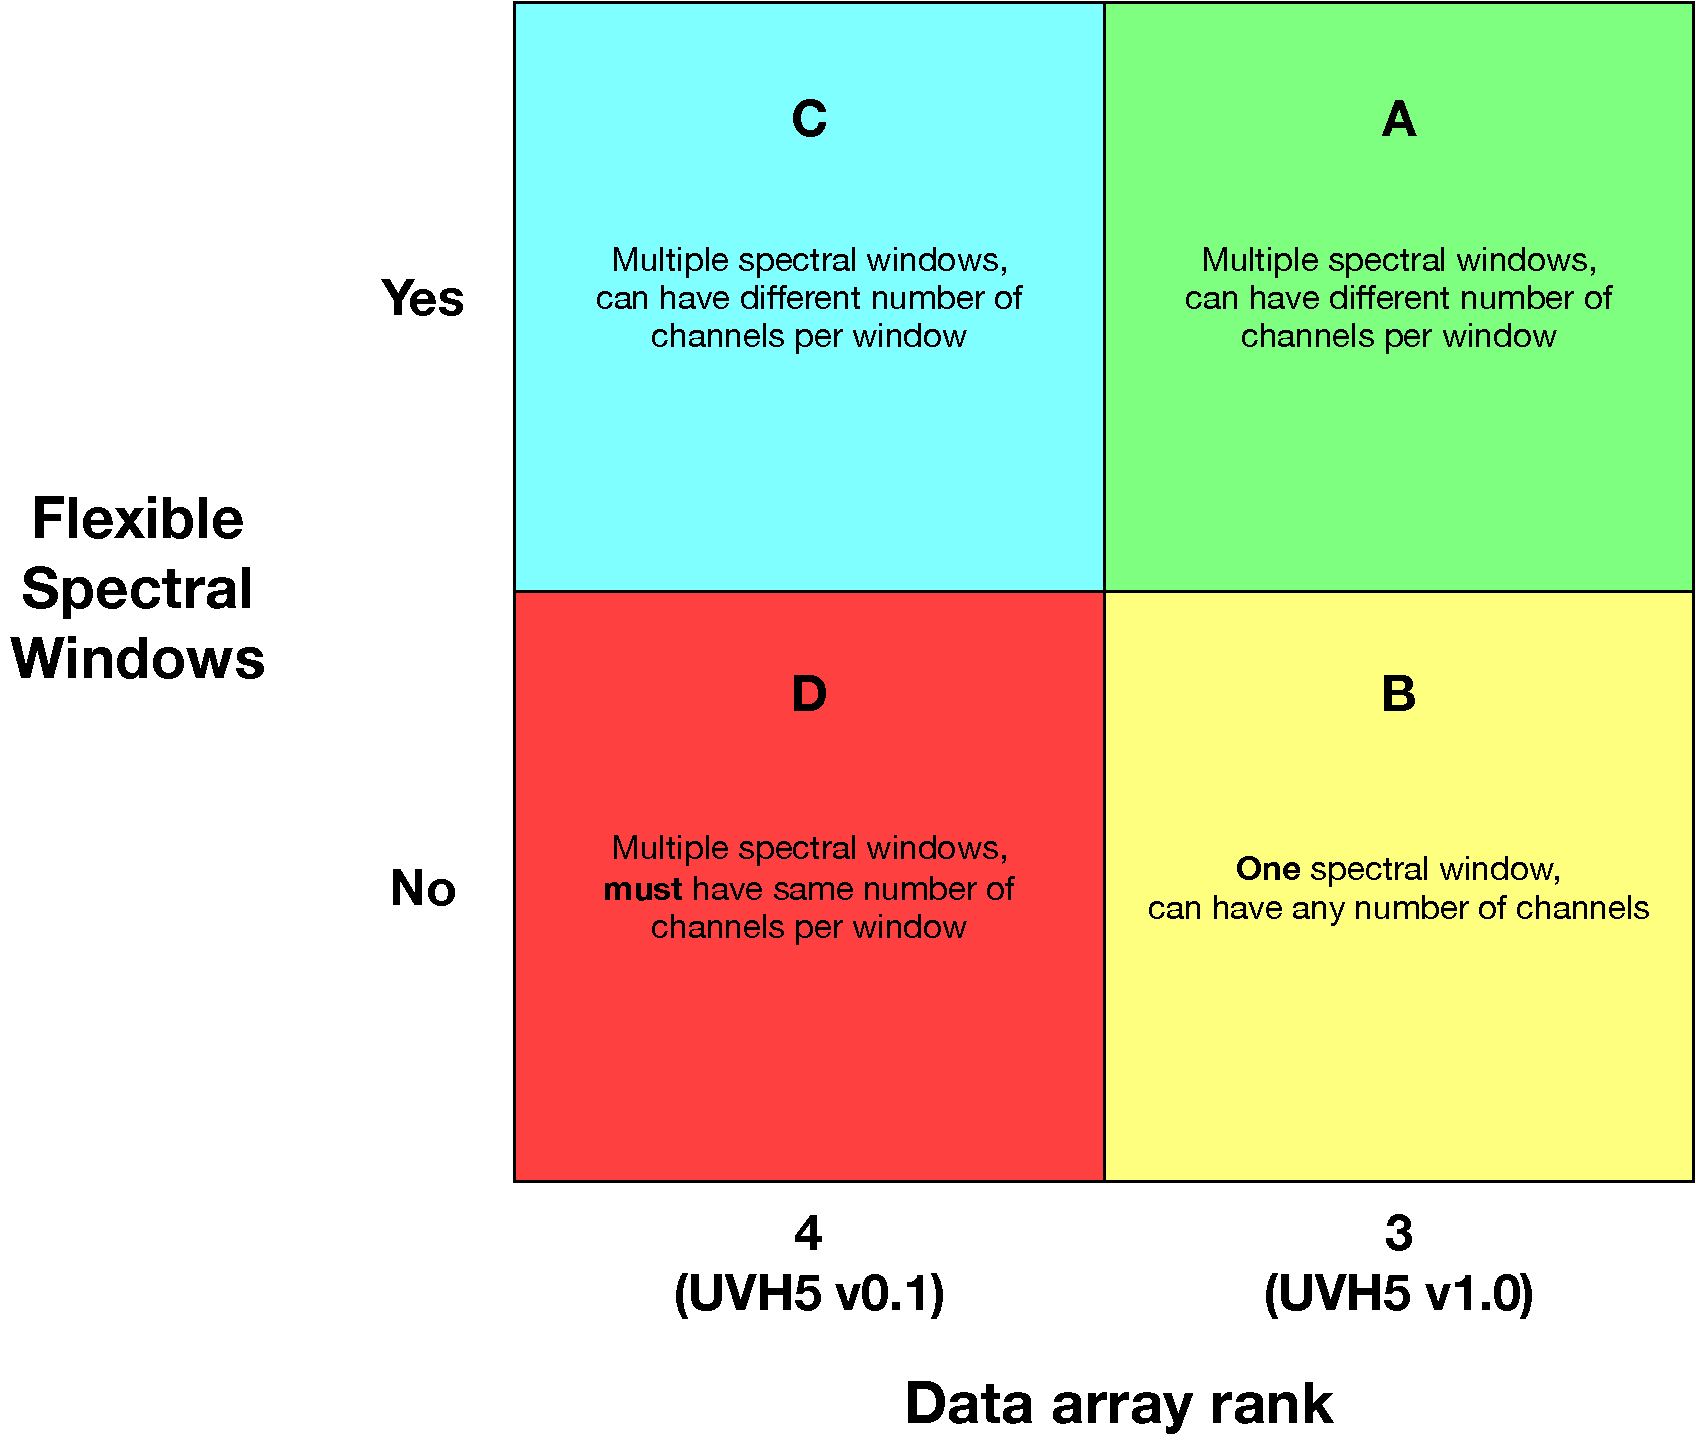
\includegraphics[width=0.95\textwidth]{uvh5_diagram.pdf}
    \caption{A summary of the different combinations of the rank of data arrays
      (reflected by UVH5 version), and flexible spectral windows. The various
      data and metadata values and ranks are listed in detail in
      Table~\ref{table:spw}.}
    \label{fig:spws}
  \end{center}
\end{figure}

To overcome these limitations, taking inspiration from how frequency data are
stored in MIRIAD, the idea of ``flexible spectral windows'' was adopted to save
the frequency information. Analogously to how baselines and times are collapsed
to a ``baseline-time axis'', frequencies and spectral windows are collapsed to a
``frequency-spectral window'' axis. This allows for more versatility in how data
from different spectral windows are stored inside of a single file, but it
requires the change of several important components of metadata. We summarize
these changes here.
\begin{itemize}
\item The value for \verb+Nfreqs+ is the total number of frequency channels
  saved in the data across all spectral windows.
\item Where required, the number of spectral windows \verb+Nspws+ is required to
  be 1.
\item The \verb+channel_width+ dataset was changed from a single number to a 1-d
  array of length \verb+Nfreqs+.
\item The \verb+flex_spw+ dataset was added to identify whether the file in
  question supports flexible spectral windows (if \verb+True+) or not (if
  \verb+False+).
\item The \verb+flex_spw_id_array+ dataset was added to identify which spectral
  window a given channel belongs. This is required if \texttt{flex\_spw} is
  \texttt{True}.
\end{itemize}

It is possible to save files self-consistently without using flexible spectral
windows \textit{if and only if there is a single spectral window}. We outline
the various (valid) combinations below in Sec.~\ref{sec:version_table}.


\subsection{Version 1.0}

\subsubsection{Rank-3 Array Convention}
\label{sec:rank3_arrays}
Version 1.0 of UVH5 represents a significant change in the way that the data
arrays (\verb+visdata+, \verb+flags+, and \verb+nsamples+) and metadata arrays
are stored. The previously vestigial spectral-window axis is removed, meaning
that data arrays are rank-3 instead of rank-4. Explicitly, these arrays have
shape (Nblts, Nfreqs, Npols), where Nfreqs includes the number of channels
across all spectral windows. This also affects the \textit{freq\_array} dataset,
which went from a rank-2 array to rank-1 of size (Nfreqs). The description of
data and metadata in the body of this memo assumes the Version 1.0
specification. Although \verb+pyuvdata+ plans to indefinitely support files
written with the previous convention (i.e., having an explicit spectral
window-axis), UVH5 files should be written such that they conform to Version
1.0.

\subsection{Table Summarizing Changes}
\label{sec:version_table}
In the interest of summarizing all of the historical changes in a single place,
we outline below the changes that have occurred in the UVH5 specification. We
note what they are currently, along with how they were saved
previously.

\begin{center}
  \begin{tabular}{ m{8em} | m{10em} | m{10em} | m{4em} }
    \textbf{Dataset} & \makecell[cl]{\textbf{Current}\\\textbf{Convention}} & \makecell[cl]{\textbf{Previous}\\\textbf{Convention}} & \textbf{Version Changed} \\\hline\hline
    \texttt{Header/version} & String corresponding to version & Not present & v0.1 \\[1em] \hline
    \makecell[tl]{\texttt{Header/}\\\texttt{integration\_time}} & Array of float, shape (Nblts) & Single float (assumed to apply to all baseline-times) & v0.1 \\[1.75em]
  \end{tabular}
\end{center}

We also summarize the combination of data and metadata properties for the cases
of: (A) rank-3 data arrays, flexible spectral windows; (B) rank-3 data arrays,
no flexible spectral windows; (C) rank-4 data arrays, flexible spectral windows;
(D) rank-4 data arrays, no flexible spectral windows. See Figure~\ref{fig:spws}
for a visual representation. \textbf{Note that we include the following only as
  a reference! We encourage UVH5 writers to conform as much as possible to the
  v1.0 specification (options A or B).}

\begin{table}[t]
  \scriptsize
  \begin{center}
    \begin{tabular}{ m{8em} | m{10em} | m{10em} | m{10em} | m{10em}}
      \textbf{Dataset} & \textbf{Type A} & \textbf{Type B} & \textbf{Type C} & \textbf{Type D} \\ \hline\hline
      \texttt{Header/Nspws} & Number of spectral windows & 1 & Number of spectral windows & Number of spectral windows \\ \hline
      \texttt{Header/Nfreqs} & Number of frequencies across all spectral windows & Number of frequencies & Number of frequencies across all spectral windows & Number of frequencies \textit{per} spectral window \\ \hline
      \makecell[cl]{\texttt{Header/}\\\texttt{channel\_width}} & Shape (Nfreqs) & Shape (Nfreqs) & Shape (Nfreqs) & Scalar (assumed to apply to all frequencies) \\[1.75em] \hline
      \makecell[cl]{\texttt{Header/}\\\texttt{flex\_spw\_id\_array}} & Shape (Nfreqs) & Not present & Shape (Nfreqs) & Not present \\[1.75em] \hline
      \texttt{Header/flex\_spw} & \texttt{True} & \texttt{False} & \texttt{True} & \texttt{False} \textbf{OR} not present \\[1.75em] \hline
      \makecell[cl]{\texttt{Header/}\\\texttt{freq\_array}} & Shape (Nfreqs) & Shape (Nfreqs) & Shape (Nfreqs) & Shape (Nspws, Nfreqs) \\[1.75em] \hline
      \texttt{Data/visdata} & Shape (Nblts, Nfreqs, Npols) & Shape (Nblts, Nfreqs, Npols) & Shape (Nblts, 1, Nfreqs, Npols) & Shape (Nblts, Nspws, Nfreqs, Npols) \\[1.75em] \hline
      \texttt{Data/flags} & Shape (Nblts, Nfreqs, Npols) & Shape (Nblts, Nfreqs, Npols) & Shape (Nblts, 1, Nfreqs, Npols) & Shape (Nblts, Nspws, Nfreqs, Npols) \\[1.75em] \hline
      \texttt{Data/nsamples} & Shape (Nblts, Nfreqs, Npols) & Shape (Nblts, Nfreqs, Npols) & Shape (Nblts, 1, Nfreqs, Npols) & Shape (Nblts, Nspws, Nfreqs, Npols) \\
    \end{tabular}
  \end{center}
  \caption{A table summarizing the different data and metadata values for
    different file types. Type A, B, C, and D refer to the combinations of data
    array rank and flexible spectral windows in Figure~\ref{fig:spws}. Note that
    UVH5 writers are strongly encouraged to write files compatible with Type A
    or B (i.e., UVH5 v1.0), whereas readers are encouraged to be as flexible as
    possible (within reason).}
  \label{table:spw}
\end{table}

\begin{thebibliography}{9}

\bibitem{tms} A.~Richard~Thompson, James~M.~Moran, and George~W.~Swenson,~Jr.,
  ``Interferometry and Synthesis in Radio Astronomy, 3rd Edition'', 2017.

\end{thebibliography}

\newpage

\begin{appendices}
\section{Strings in HDF5}
\label{appendix:strings}
String datatypes are finicky, and require special handling to ensure that they
are compatible with the HDF5 bindings in various languages. This is especially
true for files written from \verb+h5py+, which handles strings differently
between python2 and python3. Though python2 is nearing its end-of-life, UVH5
should be backwards compatible with older versions of \verb+h5py+ as much as
possible. To help service this, all string-type metadata in UVH5 files
\textit{must} be fixed-length ASCII type. Not only does this allow for
interoperability between different \verb+h5py+ versions, but it also ensures
that strings can be round-tripped through other HDF5 bindings, such as those in
C, MATLAB, IDL, Fortran\footnote{Strings in Fortran are not null-terminated, so
  these require special handling.}, etc. Note that the string should use one
byte per character, and be null-terminated. This corresponds to the numpy
\verb+S+ datatype in both versions of python2 and python3.

When writing a string-like dataset from \verb+h5py+, scalar data should be
written by casting a string to a \verb+numpy.string_+ object. Array data should
be written as a \verb+S<n>+ dataset, where \verb+<n>+ represents the length of
the strings to be saved. Upon reading, strings can be cast to bytes using the
\verb+tostring()+ method, at which point the data is \verb+<str>+-type (python2)
or can be decoded as UTF-8 to become \verb+<str>+-type (python3).

Below is an example for how to read and write string scalar and array-type
datasets using \verb+h5py+ in python2 and python3.

\subsection{Target String Type}
The following is the output of \texttt{h5dump} for a string-like dataset in a
UVH5 file. UVH5 writers are strongly encouraged (though not required) to follow
the same convention. Although something like UTF-8 is more flexible, restricting
strings to ASCII allows for greater interoperability with other file formats
such as MIRIAD and UVFITS.

\begin{verbatim}
$ h5dump -V
h5dump: Version 1.12.0
$ h5dump -d Header/history -A simulated_bda_file.uvh5
HDF5 "simulated_bda_file.uvh5" {
DATASET "Header/history" {
   DATATYPE  H5T_STRING {
      STRSIZE 1035;
      STRPAD H5T_STR_NULLPAD;
      CSET H5T_CSET_ASCII;
      CTYPE H5T_C_S1;
   }
   DATASPACE  SCALAR
}
}
\end{verbatim}

\subsection{Writing strings in python2}
\begin{minted}{python}
import numpy as np
import h5py
# open file and write string datasets
with h5py.File('test_file.uvh5', 'w') as f:
    header = f.create_group('Header')
    # scalar dataset
    header['scalar_string'] = np.string_('Hello world!')

    # array dataset
    str_array = np.array(['hello', 'world'])
    n_words = len(str_array)
    max_len_words = np.amax([len(n) for n in str_array])
    dtype = "S{:d}".format(max_len_words)
    header.create_dataset('array_string', (n_words,), dtype=dtype,
                          data=str_array)

# read the data back in again
with h5py.File('test_file.uvh5', 'r') as f:
    header = f['Header']
    # read scalar dataset
    scalar_string = header['scalar_string'][()].tobytes()
    assert scalar_string == 'Hello world!'

    # read array dataset
    str_array_file = [n.tobytes() for n in header['array_string'][()]]
    assert np.all(str_array_file == str_array)
\end{minted}

\subsection{Writing strings in python3}
\begin{minted}{python}
import numpy as np
import h5py
# open file and write string datasets
with h5py.File('test_file.uvh5', 'w') as f:
    header = f.create_group('Header')
    # scalar dataset
    header['scalar_string'] = np.string_('Hello world!')

    # array dataset
    str_array = ['hello', 'world']
    header['array_string'] = np.string_(str_array)

# read the data back in again
with h5py.File('test_file.uvh5', 'r') as f:
    header = f['Header']
    # read scalar dataset
    scalar_string = header['scalar_string'][()].tobytes().decode('UTF-8')
    assert scalar_string == 'Hello world!'

    # read array dataset
    str_array_file = [n.tobytes().decode('UTF-8')
                      for n in header['array_string'][()]]
    assert np.all(str_array_file == str_array)
\end{minted}


\section{Integer Datatype Support for Visibility Data}
\label{appendix:integers}
The HERA correlator writes datasets which have 32-bit integer real and imaginary
components. Due to the self-describing nature of HDF5 datasets, this information
is captured by the file format. Nevertheless, special handling must be used to
interpret these datasets as complex numbers. The \verb+astype+ context manager
in \verb+h5py+ is used to convert the datatype on the fly from integers to
complex numbers. Below is an example of how to do this.

\begin{minted}{python}
import numpy as np
import h5py
# define integer datatype
int_dtype = np.dtype([('r', '<i4'), ('i', '<i4')])

# open file and read in the dataset
with h5py.File('test_file.uvh5', 'r') as f:
    visdata = f['Data/visdata']
    dshape = visdata.shape
    data = np.empty(dshape, dtype=np.complex128)
    with visdata.astype(int_dtype):
        data.real = visdata['r'][:, :, :]
        data.imag = visdata['i'][:, :, :]
\end{minted}


\section{Defining Python Boolean Types in C}
\label{appendix:boolean}
As mentioned in Sec.~\ref{sec:flags}, the flags array in a UVH5 file uses an
HDF5 enum datatype to encode the \verb+h5py+ boolean type. When creating such a
datatype using \verb+h5py+, the user simply needs to ensure the datatype is
\verb+np.bool_+. The building of the enum is transparent. When building the enum
from a different language, the precise specification is necessary to ensure
compatibility. The following code is a template for how to build the appropriate
datatype using C. The construction in other languages, such as Fortran, should
follow analogously.
\begin{minted}{c}
#include <hdf5.h>

#define CPTR(VAR,CONST) ((VAR)=(CONST),&(VAR))

typedef enum {
  FALSE,
  TRUE
} bool_t;

int main() {
  bool_t val;
  static hid_t boolenumtype;
  hid_t file_id, dspace_id, flags_id;
  herr_t status;

  /* define enum type */
  boolenumtype = H5Tcreate(H5T_ENUM, sizeof(bool_t));
  H5Tenum_insert(boolenumtype, "FALSE", CPTR(val, FALSE ));
  H5Tenum_insert(boolenumtype, "TRUE" , CPTR(val, TRUE  ));

  /* open a new file */
  file_id = H5Fcreate("test_file.h5", H5F_ACC_TRUNC, H5P_DEFAULT, H5P_DEFAULT);

  /* define array dimensions */
  int Nblts = 10;
  int Nfreqs = 16;
  int Npols = 4;
  hsize_t dims[3] = {Nblts, Nfreqs, Npols};

  /* initialize data array with FALSE values */
  bool_t data[Nblts][Nfreqs][Npols];
  for (int i=0; i<Nblts; i++) {
    for (int j=0; j<Nfreqs; j++) {
      for (int k=0; k<Npols; k++) {
        data[i][j][k] = FALSE;
      }
    }
  }

  /* make dataspace and write out data */
  dspace_id = H5Screate_simple(3, dims, dims);
  flags_id = H5Dcreate(file_id, "flags", boolenumtype, dspace_id,
                       H5P_DEFAULT, H5P_DEFAULT, H5P_DEFAULT);
  status = H5Dwrite(flags_id, boolenumtype, H5S_ALL, H5S_ALL,
                    H5P_DEFAULT, data);

  /* close down */
  H5Dclose(flags_id);
  H5Sclose(dspace_id);
  H5Fclose(file_id);
  return 0;
}
\end{minted}


\end{appendices}

\end{document}


% Local Variables:
% TeX-command-extra-options: "-shell-escape"
% End:
